\documentclass[lang=cn,newtx,10pt,scheme=chinese]{elegantbook}

\title{时光剪影:我的全球观察与见证}
%\subtitle{当代历史的个人记录与评论}

\author{Anonymous}
%\institute{佚名}
\date{2024/08/19}
\version{0.1}
\bioinfo{书籍简介}{本书是从个人视角记录时代脉动的独特作品。}

%\extrainfo{注意:本模板自 2023 年 1 月 1 日开始,不再更新和维护!}

\setcounter{tocdepth}{3}

%\logo{logo-blue.png}
\cover{images/cover.jpeg}

% 本文档命令
\usepackage{array}
\newcommand{\ccr}[1]{\makecell{{\color{#1}\rule{1cm}{1cm}}}}

% 修改标题页的橙色带
\definecolor{customcolor}{RGB}{32,178,170}
\colorlet{coverlinecolor}{customcolor}
\usepackage{cprotect}

\addbibresource[location=local]{reference.bib} % 参考文献,不要删除

\begin{document}

\maketitle
\frontmatter

\tableofcontents

\mainmatter

\chapter{序言}
%《时光剪影:我的全球观察与见证》是一部从个人视角记录时代脉动的独特作品。作者通过自己的眼睛和心灵,捕捉了国内外的重大事件,并将这些瞬间化为深刻的思考与见证。书中穿插着个人体验与全球动态的交织,既有对历史的铭刻,也有对未来的展望。在纷繁复杂的世界中,作者以独到的见解为读者呈现了一幅跨越时空的全景图,带领读者穿越时光,回顾那些塑造我们当下与未来的重要时刻。

生活在这个信息爆炸的时代,世界的脉动变得前所未有的清晰,每一天都仿佛是历史书写的新篇章。面对不断涌现的新闻和事件,我们每个人都是见证者,同时也是历史的参与者。正是怀着这样的感受,我开始了《时光剪影:我的全球观察与见证》的写作。

\begin{itemize}
\item 记录时代,思考未来 \\
本书的核心目的在于记录和反思。时代的洪流裹挟着无数重要的瞬间,有些我们目睹了却很快被遗忘,有些则深深嵌入我们的记忆中,久久不能散去。我希望通过个人的视角,把这些闪光的片段串联成线,构建出一幅时代的剪影。在这些事件中,不仅有全球视野下的动荡与变迁,也有发生在我们身边的每一个微小但深刻的变化。

\item 个人与历史的对话 \\
这不是一部简单的新闻记录,也不仅仅是事实的堆积。每一个事件在我的书写中,都是一场个人与历史的对话。我试图透过现象看本质,剖析事件背后的驱动力和影响力,同时将我的思考、疑问与感悟融入其中。这样的叙述,既是对事件的忠实记录,也是对自己内心世界的揭示。

\item 全球视野与本土情怀 \\
在这本书中,国际与国内的事件交相辉映。全球视野让我们看见了大国博弈、文化碰撞与技术革命,而本土情怀则使我们感受到社会变迁、民生改善与文化传承。这些事件在时间与空间的交汇中,共同塑造了我们的现实生活,也影响着未来的走向。

\item 展望与启迪 \\
写作的过程也是思考与自我探索的过程。回顾这些年来的风云变幻,我更加确信,每一个时代都有其独特的使命与挑战,而我们所经历的正是这样一个充满机遇与风险的时代。希望本书能带给读者一些启迪,促使大家在回顾过往的同时,更多地思考未来。毕竟,历史的记录不仅是为了铭记,更是为了展望。
\end{itemize}


\chapter{新冠疫情后的~2024}

从中国的角度来看,2024年是新冠疫情封控全面放开后的第一年。2024年本是充满希望的一年,因为摆脱了疫情的束缚,我们终于又可以展开手脚,准备大干一场。。。

\section{全球大选}

2024 是有史以来最大的选举年,全球范围内数十个国家和地区举行了选举。据不完全统计,2024 年全球有超过 76 个国家和地区举行了大选,涉及北美、欧洲、南亚等,覆盖超过 41.7 亿人口,占世界总人口的比例超过 41\%,GDP 占比超过 42\%。 

从中国人的角度来说,台湾地区选举和美国大选是对我们深远影响的两个地区和国家选举,且一个在 2024 年初,一个在 2024 年底,几乎贯穿整个 2024 年。

\subsection{台湾地区选举}

台湾地区领导人和立法机构选举在 2024 年 1 月 13 日落下帷幕。民进党候选人赖清德、萧美琴当选台湾地区总统和副总统。在得票数和得票率方面,民进党候选人赖清德和萧美琴获得 5,586,019 张选票,得票率为 40.05\%,国民党的侯友宜、赵少康获得 4,671,021 张选票,得票率为 33.49\%,民众党的柯文哲、吴欣盈获得 3,690,466 张选票,得票率为 26.46\%。台湾地区立法机构共有 113 个席位,其中国民党获 52 席,民进党获 51 席,民众党获 8 席,无党籍和未经政党推荐者获 2 席。从绝对席位上来说,任何政党都没有获得绝对多数。然而,国民党和民众党席位总数为 60 席,占绝对多数。此次选举,民进党打破了台湾地区领导人选举自 1996 年以来每八年政党轮替的惯例。但是,民进党在立法机构也沦为第二大党。

赖清德具有深绿背景,并且在 2017 年 9 月担任台湾行政管理机构负责人时宣称自己“是主张‘台湾独立’的政治工作者,也是务实的‘台独主义者’”。因此从两岸关系看,赖清德的当选无疑升高了未来四年两岸关系的风险。2024 年 5 月 20 日赖清德总统宣誓就职。作为回应,中国人民解放军东部战区于 2024 年 5 月 23 日至 24 日在台湾岛周边开展由战区陆军、海军、空军和火箭军等兵种组成“联合利剑 - 2024A”军事演习,重点演练联合海空战备警巡、联合夺取战场综合控制权、联合精打要害目标等科目,舰机抵近台岛周边战巡,岛链内外一体联动,检验战区部队联合作战实战能力。这也是对“台独”分裂势力谋“独”行径的有力惩戒,对外部势力干涉挑衅的严重警告。

\subsection{美国大选}

美国总统的选举则颇具戏剧性。初期,民主党和共和党候选人分别是现任总统拜登和前总统特朗普。然而,后期对拜登健康状态的担忧,民主党候选人由拜登更换为现任副总统哈里斯。

另一个颇具影响力甚至是可能对最终选举结果产生决定性影响的是特朗普遭遇枪击事件。

当地时间 2024 年 7 月 13 日 18 时 15 分许,美国前总统特朗普在宾夕法尼亚州举行竞选集会发表演讲时,一名枪手从集会现场外高处向特朗普所在的演讲台“开了数枪”,子弹击中特朗普的右耳。其余的子弹伤及三名无辜群众,造成包括枪手在内的 2 人死亡 2 人重伤。特朗普满脸是血,随后立即撤离了演讲台。该枪手被特勤局人员当场击毙。
执法官员表示,此次枪击事件被定性为“暗杀未遂”,已作为刺杀案调查处理。当地时间 2024 年 7 月 14 日,特朗普竞选团队称,特朗普情况良好。同日,美国联邦调查局(FBI)在一份声明中表示,已确认枪击特朗普的枪手为 20 岁的美国宾夕法尼亚州男子托马斯·马修·克鲁克斯(Thomas Matthew Crooks)。 袭击特朗普的枪手是独自作案,作案动机还不清楚。


\begin{figure}[htbp]
  \centering
  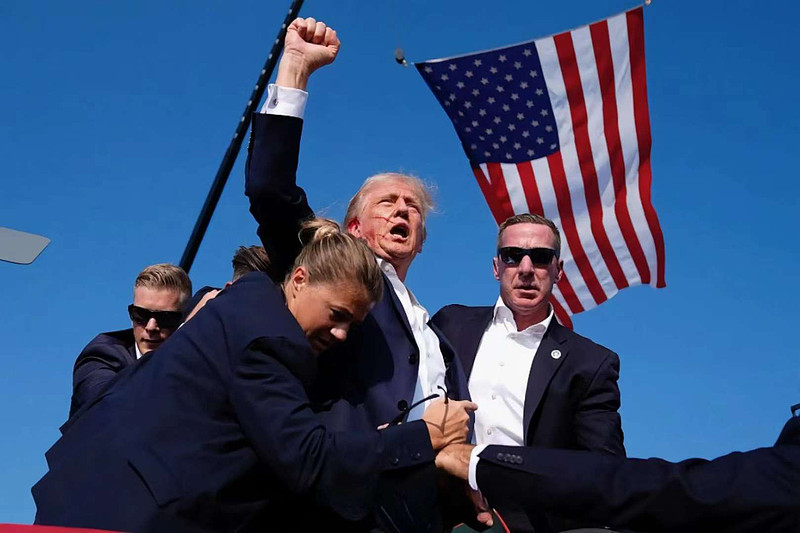
\includegraphics[width=0.5\linewidth]{./images/trump_shoot.jpg}
  \caption{特朗普枪击后照片}\label{fig:trump_shoot}
\end{figure}

图~\ref{fig:trump_shoot} 展示了特朗普遭遇枪击后的照片。尽管特勤局人员在尝试将特朗普带离现场,但特朗普仍然在大喊 fight。也许正式这种无畏的精神,激励了美国民众,促成了特朗普的再次当选。

当地时间 2024 年 11 月 6 日,根据多家美媒最新公布的初步测算,特朗普已获得 295 张选举人票超过胜选所需的 270 张选举人票提前锁定胜局,而哈里斯得票数暂为 226 张。 同日,特朗普宣布在 2024 年总统选举中获胜,哈里斯承认败选。 当地时间 11 月 9 日,美国亚利桑那州选票结果最终出炉,当选总统特朗普获胜并取得 11 张选举人票,总计获得 312 张选举人票,而哈里斯则获得 226 张。

\section{底层的动荡}

经济的下行导致社会底层动荡不断,2024年发生多起恶行群体伤害事件。

2024年8月28日13时许,王某(女)驾车行至崂山区青山村观景台附近时逆行,因对向正常行驶的林某某(男)未对其进行让行,王某下车对林某某进行了辱骂、殴打。公安机关依法对王某并处行政拘留10日,罚款1000元。

2024年9月18日,深圳日本人学校的一名学生在上学途中被歹徒持刀伤害,最终抢救无效于19日凌晨去世。记者从深圳警方获悉,经调查,该案属偶发个案,犯罪嫌疑人钟某对持刀伤害学生行为供认不讳,已被依法刑拘,案件正在进一步侦办中。

9月19日,湖南省财政厅党组书记、厅长刘文杰在其居住的住宅楼意外坠楼死亡,同时间段坠楼死亡的还有另外两名男子。

10月1日凌晨,澎湃新闻记者从上海松江公安分局获悉,2024年9月30日21时47分,松江公安分局接报警称,松汇中路某超市内有一男子持刀伤人。接报后,民警迅速到场,犯罪嫌疑人林某某(男,37岁) 被当场抓获,18名受伤人员马上送医救治,其中3名伤者抢救无效死亡,其余伤者无生命危险。据初步侦查,林某某因个人经济纠纷,来沪泄愤实施上述行为。案件在进一步侦办中。

10月8日下午2点左右,在广州天河区华强路第一小学华穗校区的校门外路段,涌现了很多刚从兴趣班放学的孩子,以及一部分中午在家休息完下午返校上学的孩子。可是没想到,就在这时,人群里突然冲出一名60岁左右的男子,掏出一把小刀,对着过往的小学生人群,就是一顿乱捅乱砍。有几个小学生因为毫无防备,不幸被砍伤。男子的砍人行为,造成了三人受伤的后果。

2024年10月28日15时20分许,海淀区万泉庄路和万柳中路交叉口附近,发生一起持刀伤人案件,导致5名路人受伤,其中3名未成年人。犯罪嫌疑人唐某某(男,50岁)被当场控制,伤者及时送医治疗,无生命危险。目前,案件正在进一步调查中。

2024年11月11日19时48分许,一辆小汽车在广东省珠海市香洲区体育中心撞倒多名行人后驾车逃逸。警方接报后迅速派员到场处置,并协助将伤者送往医院救治 [1]。珠海市公安局香洲分局通报称,司机樊某(男,62岁)已被警方控制 。2024年11月12日,珠海市公安局发布警情通报,案件致35人死亡,43人受伤。 [4]案件发生后,中共中央总书记、国家主席、中央军委主席习近平高度重视并作出重要指示。

\section{油罐车混装食用油}

新京报报道称,在5月份追踪调查中发现有两辆刚卸完煤制油的罐车,在并未洗罐的情况下,顺利装上了食用油,涉及的食用油企业分别是汇福粮油集团和中储粮油脂(天津)有限公司。此外,报道还称,国内许多普货罐车运输的液体并不固定,既承接糖浆、大豆油等可食用液体,也运送煤制油等化工类液体。

7月9日晚最新消息,针对媒体反映的“罐车运输食用油乱象问题”,国务院食安办高度重视,组织国家发展改革委、公安部、交通运输部、市场监管总局、国家粮食和储备局等部门召开专题会议研究,成立联合调查组彻查食用油罐车运输环节有关问题。对于违法企业和相关责任人,将依法严惩、绝不姑息。同时举一反三,组织开展食用油风险隐患专项排查。调查处置结果将及时公布。

8月25日,针对媒体反映的“罐车运输食用植物油乱象问题”,国务院食安办、国家发展改革委、公安部、交通运输部、国家卫生健康委、市场监管总局、国家粮食和储备局组成联合调查组,分赴河北、天津、内蒙古、陕西四地开展联合调查,追查涉事产品流向,核查涉事责任人员及责任单位的违法行为,分析问题原因,理清各方责任。同时,在全国范围内组织开展全链条清理排查,从各地清查情况看,截至目前,未发现其他同类问题。

联合调查组经调查核实后认定,罐车混运食用植物油事件性质极其恶劣,违反基本常识,践踏道德底线和法律红线,是典型的行为违法犯罪,必须严厉打击。

具体调查报告如下。

一、违法事实

涉事罐车冀 E5476W 相关违法违规事实。5月22日11时,司机要某某驾驶涉事罐车从宁夏煤业有限责任公司煤制油分公司装载煤制油,5月23日16时到达河北石家庄晋州市华力油脂有限公司,卸载全部货品。5月23日21时到达河北省衡水市武强县休息,5月24日16时从中储粮油脂(天津)有限公司装载食用植物油,5月24日21时到达河北省沧州市献县休息,5月25日21时到达山西省临汾市洪洞县休息,5月26日17时到达陕西省汉中市勉县休息,5月27日7时到达陕西勉县新力油脂有限公司,卸载油品35.91吨。经查,7月3日,涉事车辆(登记在河北邢台金谷仓物流有限公司名下)的实际车主高某群为掩盖问题,指使其三哥高某修伙同河北邢台金谷仓物流有限公司负责人孙某某,找到河北石家庄民通汽车服务有限公司负责人胡某某开具5月23日罐车清洗虚假票据(500元)。

涉事罐车冀E6365Z相关违法违规事实。5月16日17时,司机张某某驾驶涉事罐车从宁夏煤业有限责任公司煤制油分公司装载煤制油,5月18日16时到达河北省秦皇岛衡杉科技有限公司,卸载全部货品。5月19日19时到达河北省秦皇岛市海港区等待配货,5月20日19时到达河北三河汇福粮油集团精炼植物油有限公司等待装车,5月21日11时从河北三河汇福粮油集团精炼植物油有限公司装载食用植物油,5月22日12时到达内蒙古鄂尔多斯市东胜区百胜隆粮油有限公司,卸载油品31.86吨。司机张某某称5月20日已做清罐处理,经公安机关现场核查,当时涉事罐车轨迹所在地周边没有符合专业要求的洗车店和移动清洗车。

二、流向追查

涉事罐车冀E5476W所运35.91吨油品,用于饲料加工11吨,其余24.91吨未售出,已全部封存。涉事罐车冀E6365Z所运31.86吨油品,已封存2.48吨;剩余29.38吨被分装销售,其中5月22日分装8.5升规格580桶4.5吨、17升规格180桶2.79吨,5月28日分装8.5升规格280桶2.17吨、17升规格310桶4.81吨,6月10日分装8.5升规格490桶3.8吨、17升规格729桶11.31吨,总计8.5升规格1350桶10.47吨、17升规格1219桶18.91吨。已销售但未被使用的7.78吨已全部追回并封存,已被使用的21.6吨流向内蒙古鄂尔多斯市,未流向其他地区。

三、责任认定

我国《食品安全法》《粮食流通管理条例》等法律法规,以及《食品生产通用卫生规范》《食品经营过程卫生规范》《食用植物油及其制品生产卫生规范》等强制性国家标准有明确规定,要求“贮存、运输和装卸食品的容器、工器具和设备应当安全、无害,保持清洁;不得将食品与有毒、有害、或有异味的物品一同贮存运输”“运输食品应使用专用运输工具;食品运输工具不得运输有毒有害物质,防止食品污染”“运输食用植物油及其制品的车、船等运输工具、容器应符合国家相关法规标准的要求”。但一些企业和个人违反基本常识,践踏道德底线和法律红线,性质极其恶劣,是典型的行为违法犯罪。

联合调查组认定,运输企业负有管理责任,依据《食品安全法》《道路运输条例》给予行政处罚;车主负有主要责任,涉嫌犯罪的依法移送公安机关;司机负有直接责任,应以行为犯论处,依据《刑法》有关条款追究刑事责任;购买企业作为委托运输方负有相应责任,应依据《食品安全法》给予行政处罚;生产企业通过销售合同约定将运输和交付环节责任全部由买方承担,违反《食品安全法》有关食品生产经营者应当保证食品安全、对社会和公众负责的规定,应给予行政处罚。

涉事地区人民政府责成相关行政部门,对河北邢台卓然联合运输车队法定代表人倪某某、河北邢台皓源物流有限公司法定代表人澹台某某、河北邢台金谷仓物流有限公司法定代表人陈某某,罐车冀E5476W实际车主高某群、罐车冀E6365Z实际车主刘某某等5人依法查处,对构成犯罪的移送公安机关依法追究刑事责任。公安机关对涉事司机要某某、张某某,依法刑事立案并采取刑事强制措施。对参与开具罐车清洗虚假票据的河北邢台金谷仓物流有限公司负责人孙某某、河北石家庄民通汽车服务有限公司负责人胡某某、罐车冀E5476W实际车主的三哥高某修等3人,依法处以10日拘留的行政处罚。

依法对涉事7家企业给予行政处罚:对河北邢台卓然联合运输车队,依法收缴道路运输经营许可,处罚没款合计约168万元;对河北邢台皓源物流有限公司,依法收缴道路运输经营许可,处罚没款合计约151万元;对河北邢台金谷仓物流有限公司,依法处罚没款合计约192万元;对陕西勉县新力油脂有限公司,依法给予警告,没收违法所得约30万元;对内蒙古鄂尔多斯市东胜区百胜隆粮油有限公司,依法给予警告,没收违法所得约26万元;对中储粮油脂(天津)有限公司依法处罚款约286万元;对河北三河汇福粮油集团精炼植物油有限公司依法处罚款约251万元。

涉事地区河北邢台是问题罐车所在地,对罐车运输失管失察,市政府分管负责同志负有领导责任,相关监管部门人员负有责任,由地方纪检监察机关依法依规追责问责。对调查过程中地方发现的公职人员可能存在的失职渎职不作为问题,由当地纪检监察机关介入调查。

下一步国务院食安办按照全面清查、举一反三、打建结合、标本兼治的原则,会同国家粮食和储备局、交通运输部、市场监管总局等部门,持续深入开展罐车运输食用植物油问题专项整治,严格落实食用植物油运输专车专用,以“零容忍”的态度,严处重罚各类违法违规行为,加强全链条管理,健全完善监管协调机制,确保食用植物油安全。欢迎来自媒体记者、人民群众等各种方式的社会监督。

\section{洞庭湖决堤}

在遭遇2024年以来最强降雨后,洞庭湖在时隔4年后再次遭遇高洪水位。尽管日前洪峰已过,但洞庭湖标志性水文站城陵矶站2024年7月5日仍然维持警戒水位。

2024年7月5日15时32分,湖南岳阳市华容县团洲乡报险,团北堤段堤面发生塌陷;15时45分,华容县工程处险组到达现场,发现桩号19+450处堤面下陷1.5米,堤身内坡有大量出水,流量约2立方米每秒。工程组立即调集装满砂石车辆赶至现场。约10分钟后堤身缺口,面宽约5米 [1] [6]。当地网友发布的视频显示,一处堤防出现数米宽的溃口,有多辆装满沙的卡车被投入溃口中。另一段视频中,大水冲过溃口,将卡车冲走并掀翻。

2024年7月5日晚上7时,据悉,决堤口宽度已延伸至约100米。截至5日晚10时,缺口宽约8米、长约150米。到2024年7月6日6时16分,决口宽度约为225米,决口造成淹没面积约45.92平方公里。2024年7月6日7时许,人民日报记者来到湖南省岳阳市华容县团洲垸一线堤防决口区域,看到水流仍以较快流速涌入垸内,部分房屋已被水淹没至屋顶位置。在通向决口方向的洞庭湖一线大堤上,载满石块和砂石的卡车排成长队,有序驶往决口现场。

截至2024年7月6日上午9时,洞庭湖团洲垸溃口宽220米,溃口堤内外水位仅相差0.17米。当水位持平时,溃口将进行封堵,大批车辆人员在堤上待命。堤外水位为31.63米,堤内水位为31.46米,相差0.17米。溃口流速在变慢,堤内外水位均在回升,待堤内外水位持平时,施工人员将对溃口进行封堵。卫星影像显示,决堤第二天上午(7月6日9时),土黄色区域即为决堤后洪水覆盖的区域,该区域最长约13公里,最宽约5公里。

截至2024年7月6日11时,溃口处内外水位落差0.10米,长226米。截至7月6日12时许,堤坝决口宽约220米,垸内平均水深约5米,淹没面积47.64平方公里(占团洲垸总面积的92.5\%,该垸安全区暂未被淹),洞庭湖与垸内水位落差约0.10米。

截至2024年7月6日13时,决口处内外水位齐平,流速相对平缓,逐步具备了封堵决口的初步条件。

\section{尸体盗窃案}

2024年8月8日律师易胜华在新浪微博上公开一起盗窃、侮辱、故意毁坏尸体案的案件材料。

相关材料显示,2015年1月到2023年7月,山西奥瑞生物材料有限公司(简称:奥瑞生物)涉嫌通过从四川、广西、山东等地非法购买遗体、残肢作为原材料,并在购买和生产过程中对非法获取的尸体、尸骨进行处理后,用于生产“同种异体骨植入性材料”产品。

经国家审计署太原特派办审计,2015年-2023年的营业收入合计达到3.8亿元。警方在侦办该案中,查封涉案公司人体骨骼原材料、半成品18余吨,成品34077个。根据材料,该案涉及非法盗窃、倒卖尸体数千具。

该案由山西太原市公安局负责侦办,目前已将此案移送至太原市检察院审查起诉,涉案罪犯达到75人。

案件材料称,2017年至2019年期间,嫌疑人苏成忠先后以承包、入股、派人入驻等方式,控制四家殡仪馆的火化场。随后指使其安排在火化场的人员盗窃尸体,并在火化车间内对尸体粗暴肢解后,运回其公司,部分尸体在其公司内肢解,苏成忠供述上述四家火化场共向其公司提供4000余具人体骨骼。

材料称,该案共有75名犯罪嫌疑人,均对犯罪事实供认不讳,认罪认罚,涉及的单位包括奥瑞生物、四川恒普科技有限公司(下称四川恒普公司)、山东青岛大学附属医院肝脏病中心、桂林医学院、桂林市殡仪馆、平乐县殡仪馆、永福县殡仪馆等单位。

犯罪嫌疑人苏成忠所控制的云南水富市火化场、重庆巴南区仙居山火化场、贵州石阡县火化场、四川大英县火化场。

\section{死在出租屋的女孩}

2024年8月15日, 一个外地女孩,死在了我出租的公寓的公众号文章刷屏,文章内容如下。

这件事,一直想记录下来,但只要提笔就觉得沉重,不知从何写起。6月下旬平平无奇的某天,一通电话将我卷入了很长一段时间的情绪黑洞。

我的租客,死在了我的房子里,时间久到尸体已经高腐,面目难辨。

慌乱的一上午,因为我人不在西安,于是,物业、中介、开锁公司在我的授权下,打开了房门,物业全程给我拍摄视频,房门打开前的每一秒,我都祈盼是虚惊一场,但直到开锁师傅彻底将门打开,指着屋内的地板,很小声的回过头说:“人死咧”。声音轻到我要把手机声音键开到最大才能听清楚这三个字。视频也到此戛然而止。

房门再次掩住,开锁师傅离开,摆了摆手,开锁费,算了。物业报了警,一切要等警察来。警察出警不算慢,可远在新疆的我却觉得无比漫长……自杀?谋杀?突发疾病?入室杀人?又或者死者是谁,是我的租客吗?无数的疑问在我的脑海盘旋。

警察来了,法医也来了,尸体被抬走,30楼一上午的喧嚣戛然而止。

今年4月初,我在北京出差,突然接到中介电话,我在2月底委托她帮我出租的房子,有人要租,这个房子是个只有50平的单身公寓,但因为地段和装修都算好,租金不算便宜,挂出去后询问的人很多,但基本都嫌贵而一直未租出。

直到4月,我都快忘了出租这件事,却突然接到中介电话。租客很干脆,从看房到签合同,没有超过两天。当然,租客选房,我也选租客,我询问中介,租客的具体情况,信息很少但足够我放心,91年的单身女孩,从宁夏来,职业是会计,目前正在西安找工作。

看房、验房、网签合同等流程都很顺利,只是交租金时,一波三折。一开始租客问我要了支付宝账户,但没有转来,后又加了微信,也没有转来,辗转多次,我也没催,直到下午她转给我,中介说,因为输错密码导致锁卡,专门去银行办理了解锁才将钱转出。

这个细节,我当时并未在意。

粗心的我,并没有意识到。但她的死亡,从她交租金时其实就已经埋下伏笔。半年的房租,后来我才了解到都是她的母亲找村里亲友借的。如果时光倒流,我一定劝她别花这钱,回老家。可当时,她甚至对我屏蔽了朋友圈,我对她的情况,几乎一无所知。

大好年华本该是奋斗的年纪,但究竟什么是压死她的最后一根稻草?

时至今日,事情早已了结,警方也已结案,可她的生理死因,依然是个谜。就和她的骨灰、遗物最终被父亲像丢垃圾一样丢弃掉再无踪迹,永远都不会有答案了。

整理这些记忆,依然觉得内心烦乱,过程中有太多颠覆认知的地方,太多中国社会、中国农村难以触及、根深蒂固的痛点。

我该如何叙述,一个西部贫困山村女孩,经过怎样的努力,考入北京某211名校,毕业后的几年,一心考公,多次取得家乡省份事业单位笔试第一的成绩,却连连因面试环节落榜,最终又怀着怎样的失望远走他乡,依然没有找到与内心孤傲、与名校出身、与家人期望相匹配的工作,最后又是在怎样的绝望中结束了自己短暂的33岁的生命?

我也曾气愤过,气愤人要寻死,方法千千万,却为何死在租住的房子里,让我蒙受巨大损失;气愤她莫名奇妙、不留只言片语的离开,让我也背负过嫌疑。但随着案件的深入调查,我却又恨不起来,我为死者年轻生命的消逝而惋惜,也心疼死者面朝黄土背朝天一辈子却依然一贫如洗的双亲,也因西北贫困落后地区的风俗习惯而落泪,但很多时候谈起来,只有一声叹息……

尸体被法医拉走后,警方很快就联系到了她的父母。

原来她的家人,在一周前也将女儿按失踪人口报了案,他们最后一次联系到女儿,是4月20日,女儿微信问母亲要生活费,母亲表示家里确实没有钱了,要等她去借。此前的4月9日,母亲才问亲人借款1万多元转给女儿支付房租,4月21日,母亲再次找人借到1000元,转给女儿,从后续警方调查来看,这1000元还是死者母亲分两次各借500元凑的,女儿没有收,随即拉黑了所有亲人。

至此一直到她死去,都再也没有联系过任何亲人。

为什么没有收这救命的钱,反而拉黑了所有人?

答案我们永远不会知道了,只是从警方掌握的细枝末节里推测,女孩心高气傲,从小学习成绩好,村里无论谁提到她都是竖起大拇指,作为家里甚至村里的骄傲,她一是愧疚父母又因她而借钱,毕竟自己已经33岁了,还没有找到满意的工作;二是1000元杯水车薪,不是她的预期。反观她的父母,作为宁夏西海固地区、六盘山深处的农民,能把一个非独生的女孩子供到北京去读书,毕业近十年一直负担没有工作的女儿的生活开销,实在堪称伟大。

要知道,死者家乡这个县直到2019年才脱贫摘帽,而宁夏的西海固地区农村曾经也是重男轻女较为突出的地方,一个农村贫困家庭的女孩能坚持读书的不会太多,往往是很早就嫁作人妇。但在我后面与死者父亲面对面的交流中,老人透露出了对女儿厚重的期望,“她把书读下了,是我们全家的希望,甚至是村里的希望,家里就指望她了”,这里我似乎理解了女孩对考公的执着,也能感受到她巨大的压力。

直到6月初,女孩家人一直联系不到女孩,报了案。我远在新疆,一直和办案民警保持联系,对方表示我不必着急回去,目前回去了也没用,第一步要等死者父母从宁夏赶到西安后进行dna鉴定,确定死者就是我的租客。

我不断询问死者死因,警方谨慎,只告诉我死亡时间大约两周至20天,尸体高腐是因为那些天西安持续高温。而从房屋内情况初步来看,屋内整洁,门窗完好,基本可排除他杀,但还需要再次的现场勘验,并通过调取死者的电话记录、楼宇监控甚至购物记录等大量的外围调查去验证。等案件清晰明了后我再回去也不迟。

死者父母当晚就从宁夏赶到了,民警告诉我dna已经提取,2-3个工作日出结果,等结果出来,我就可以从新疆动身。死者父母目前情绪激动,无法接受。“就莫法提么”民警的话语里满是无奈。

6月的最后一天,我向单位请了长假,飞往西安。

飞机上,我的手机有三个未接来电,都是办案民警,到家已经凌晨,我给民警发去短信,我已回来,全力配合调查。

人生中第一次做笔录,是正儿八经在询问室里。其实在我回来之前,民警的外围调查就已经基本结束,我的笔录除了要使案卷更具完整性,更重要的是,死者父母坚决不同意解剖尸体查验死因,理由是家乡风俗不允许人死后无全尸。

因为不同意解剖查验死因,这起自杀事件要结案就变得异常麻烦,民警需要做大量外围调查来证明这不是一起刑事案件,办案民警也很头大,只是楼宇监控就好几个t的视频。

私下我也表示不解:尸体既已腐烂,解不解剖又有什么区别呢?除非女儿为何死去,父母其实心里是知道原因的。民警表示认同,并说出了另一个很重要的原因:死者家人从宁夏来到这里住在旅店,每天开销很大,而解剖验尸需要一定时间,他们不想等,也等不起,只想尽快了结。

也正是在民警抽丝剥茧的调查中,这个女孩最后两个多月的生活轨迹逐渐清晰呈现,那是任谁看了都会心痛的非正常生活。

我,是死者生前微信上的唯一联系人。尽管我还是被她屏蔽了朋友圈的,但也是唯一可以与她微信互发信息的人,其他仅有的几个联系人都被她拉黑。警方让我提供每次与女孩微信联系的时间和内容,因为没有删聊天记录的习惯,所有记录得以保存。

4月9日,中介让她加我微信并将半年房租转给我。我收钱后告诉她有任何问题随时联系我,同时交代她去物业进行租住人员登记并办理门禁。

4月10日,她询问我阳台的电动晾衣机使用方法,同时将我在房间装饰摆放的所有玩偶集中到酒柜里,还给我拍了照片,说她不需要这些。我说如果要使用酒柜,可自行将这些玩偶处理掉,她也表示不用酒柜。

4月17日,她给我发视频,又发语音电话,因为我正在开会就拒绝了,让她打字说,她很慌乱,说家里来了一个天然气公司的工作人员,以屋内天然气管道不合规为由,要求买保险并同时更换气管,并让我接听该工作人员的电话。我询问她有无检查对方工作证件,是否确认为天然气公司工作人员,她向对方提出此要求时,对方没有多说而是离开了。我随即联系物业,询问当日有无天然气公司人员来小区入户排查,得到否定答案。当时我第一反应是,这个女孩怎么会如此没有生活经验,感觉会很容易受骗。

联想到她身份证上的地址,那个偏远的宁夏农村,我忍不住和她说,这边不比她的老家,一个人居住凡事要多留个心眼,不害人也别被人骗,为了给她壮胆,我还告诉她,我和我爱人都是公安,如果遇到任何事,都可以咨询我。

6月3日,我收到国网陕西电力的短信,提示我电费已欠费23.17元,如果还不缴费,房屋将于6月4日13点断电。我主动联系她提醒她缴电费,如果断电了冰箱里的东西会腐烂,我是上午发信息给她,她直到下午17点才回复我:知道了姐,冰箱里没东西。

6月13日,我再次收到国网陕西电力的短信,提示我家中已欠电费24.17元,请尽快缴费。对比10天前欠费金额,只多欠了1元,我意识到房子里确实于6月4日13点前断电了,于是再次联系她,这一次,没有得到任何回应。

最后一次联系她,是6月25日,当日小区物业联系我,我们这栋楼30层有很大的臭味,经过排查,确定味道的源头就是我的房子,物业联系了房客,电话是关机状态,又联系到我,希望我能打开房门,我联想到此前她没有回复我的信息,心里隐约担忧,给她打了多个语音电话均无人接听,打手机,关机。

最终我联系了当时的中介,并委托中介、物业和开锁公司三方共同撬开门锁,结局便是开头所述,最不愿看到的事情,发生了。

做完笔录,逐字核对,最后摁上手印,需要我配合公安机关的工作算是完成了。民警提醒我,现在想删掉对方微信就可以删了。但事情远没有结束,还有最不愿意面对的事情,就是与死者家属的见面。

因为家属希望得到一些补偿,或者说人道主义的抚恤,需要和我面谈。其实那两日在派出所,我多次与死者父亲擦肩,但当时我们彼此并不知道对方是谁,民警也认为从法律上讲,我可以不直接与对方家属接触,也没有赔偿的义务。民警可以代替我带死者父母去我的房子收拾死者遗物。

但民警也多次告诉我,对方家里确确实实很贫困,从死者的生前的消费记录来看,她无论吃饭还是买任何东西,都几乎没有超过五块钱,都是买很差很差的东西凑合吃凑合用,最后一次楼宇门禁识别人脸进入是5月20几号,此后无论是监控视频还是单元门禁都没有显示她有过外出,这期间也没有点过外卖,家里也没有做饭的痕迹,电话记录也显示她没有与任何人通过话,她几乎是在极度的孤独中死去的……

联想到法医推测她的死亡时间是6月15号左右,我震惊了,民警是没有把话说透,20多天时间,独自在房间里,没有外卖没有做饭,她极大可能是把自己饿死在房间内的……我曾要求看死者父亲的笔录,被拒绝,但民警还是读了一段他借钱给女儿开销的过程,我在民警办公室就没忍住落下泪来。民警说,如果可以,给对方一点经济补偿吧。

最终,我们还是在派出所的调解室见面了。民警回避,只有我们双方到场。

对方来的是死者的父亲,以及两个远房表哥,外表都是朴实的西北男人面貌,我们聊了许多,关于死者本人的经历,关于他们的家庭状况。

女孩心气高,主意正,总想着要争口气,做事情决心大,就如她高考取得优异成绩也如她考公多次笔试第一,他的家人至今仍旧认为是考试不公,第一名都不被录取,一定是因为他们农村家庭没有背景,名额被有背景的人顶了去,字里行间对当今社会有很大怨气。

我说既然是这样果决的性格,愿望没有达成,她会不会就是已经做好了死去的准备,在她没有工作,没有收入来源的情况下,去送快递送外卖,也是能养活自己的营生,但为什么没有去做,反而是抱着不成功便成仁的心态,并且离开的如此决绝,连封遗书都没有留下。

她的父亲认为女儿的性格做得出这样的事,但他很快回到正题,既然人已经走了,死者为大,希望我作为房东能够给予一定补偿,他的老伴已经在旅店里病倒了,也急于回宁夏,事情了结后,会尽快将女儿尸体火化,然后找个地方把骨灰扔了,“就当她没来过吧。”

轻轻几个字,我感觉我的头皮都炸开了,我问他为什么扔掉骨灰?怎么舍得?以后不祭奠了吗?他轻轻哼了一声,没啥祭奠了,他们那里的风俗,女孩没嫁人就死了的,不允许进自家祖坟,即使嫁人了,没生娃就死了的,也入不了夫家祖坟,最后都是尸骨难寻。

我一时间感觉很气愤,说这些都是落后的风俗,况且风俗算什么,这是你女儿,你管他风俗不风俗,你就非埋进自己祖坟又怎样?以后也有个烧纸钱的地方。女孩的表哥说,这不是一家的事,人这样死了,村里人也不允许带回去的……

我同意了给予一定的补偿,只想尽快结束,不想再将自己缠绕在如此离奇复杂的事件中。最后一件事就是带他们去房屋内拿取女孩遗物,谈妥后我去找民警要房屋钥匙(案件结束前房屋贴了封条钥匙也由警方保管),准备带他们去拿遗物,死者其中一个表哥表示必须在出派出所前把赔偿给他们的钱转给死者父亲,他可能怕我走出去就赖账。

面对这样的不信任,我稍稍为之前的恻隐之心感到懊悔。女孩父亲打开收款码,我将钱转给他。

派出所离房子并不远,不到两站路,我提议走路前往,那天下着毛毛细雨,我们都没有撑伞,各怀心事很快就走到了楼下,我把钥匙交给他们,并把房号告诉他们,委托他们离开时把所有窗户打开,我就不上去了,在楼下等他们。

他们走后,我坐在楼下的长椅上,仰头看着30层,心里难以诉说的难过,楼下是闹市区,人群熙攘,车水马空,人们都奔赴在各自的生活中,欣欣向荣,可是这些热闹再也与短暂住在30楼的那个女孩无关了。

来来往往的人群,有人知道30楼逝去了一个年轻的生命吗?有人在乎吗?也许我会一直记住她,原因仅仅是她住过的房子未来几年都只能闲置,我也不会踏入,她带给我的直接经济损失会使我记住她吧。

可是,她来到人世一场,从西北山村考入首都北京,有过人生的高光时刻,最终却落得如此下场,是谁之过?是社会、家庭还是自身性格呢?什么是压死骆驼的最后一根稻草,我仍然没有答案。

想到等会就将与死者的家人再无往来,想到他们还要长途跋涉赶回宁夏,我去附近的便利店去买了一些水和面包,想让他们带在路上,刚出便利店就远远看到他们已经拖着一个并不大的行李箱下了楼,女孩的遗物真的少得可怜。

可下一刻,我就目睹了女孩的父亲,将那个行李箱毫不犹豫的扔进了路旁的垃圾桶,没有丝毫不舍,没有丝毫留恋,头也不回的走了。她就这样消失了,没有留下一点痕迹,是父母消失的女儿,是村里消失的骄傲,是我素未谋面的消失的房客……

我还是迎上去,将手中买的东西递给女孩的父亲,交接塑料袋提手的一霎那,我短暂的碰触到了女孩父亲的手,又像触电般收了回来。因为想到他刚刚在房间是收拾了遗物,那个房间,此前才搬运走了一具腐烂的尸体,我突然有一种难以名状的反胃。

抬头才发现,女孩的父亲满脸涨的通红,像刚喝过酒似的,双眼明显哭过,整个人的状态就是马上要哭出来的样子,连谢谢两个字都说的结结巴巴,仿佛再多说一个字,情绪就要喷涌出来。他养了30多年的女儿,他能不难过吗?可是所谓风俗甚至是迷信思想割裂了最后的亲情,他真的能放下吗,我是不信的。

道别时我想我们此生都不会再有交集了,我嘱咐他们一路平安,保重身体,在我心里,这是替他们死去的女儿向她的父亲作最后的告别。

一想到我是死去女孩唯一的联系人,我没有删掉她的微信。

\section{政府与反腐败}

中国共产党第二十届中央委员会第三次全体会议,于2024年7月15日至18日在北京举行。

12月23日,河南省安阳市中级人民法院对党志军犯故意杀人罪一案进行一审公开宣判,以故意杀人罪判处被告人党志军死刑,剥夺政治权利终身。2024年8月7日傍晚,河南漯河市郾城区法院立案庭副庭长、一级法官王佳佳被犯罪嫌疑人党某某行凶报复,不幸遇害。2024年8月7日18时26分,公安机关接报,某小区地下停车场负二层电梯口处有人被刺伤,公安机关立即赶赴现场,发现郾城区法院王佳佳法官颈部被刀割伤,已无生命体征。经查看相关录像,行凶者系王佳佳法官所办道路交通事故损害赔偿案件的原告党某某(男,50岁,漯河市郾城区居民,未婚)。2024年8月8日3时许,公安机关在党某某家中将其抓获,被抓获时党某某已畏罪服毒,处于昏迷状态,经送医治疗无生命危险。

9月5日微博视频号的报道:赖清德近日谈及俄乌冲突时,提及大陆问题,并质疑为何大陆一再强调领土完整,却没有收回在《瑷珲条约》中被俄罗斯割占的领土。

2024年9月13日第十四届全国人民代表大会常务委员会第十一次会议通过全国人民代表大会常务委员会关于实施渐进式延迟法定退休年龄的决定。

9月20日,中国表示已与日本达成协议,逐步恢复日本海鲜进口。自2023年8月24日日本启动福岛第一核电站核污染水排海以来,就没再进口日本水产品。 8月30日,俄罗斯科学院远东分院太平洋海洋研究所发布其对远东海洋海水的检测结果报告称,日本福岛第一核电站启动核污染水排海后,日本周边海水的放射性物质含量非常低,氚的含量目前不会对海洋及海洋生物构成威胁。

11月28日,国防部举行例行记者会。国防部新闻局局长、国防部新闻发言人吴谦大校发布信息称,中央军委委员、军委政治工作部上将主任苗华涉嫌严重违纪,经党中央研究,决定对苗华停职检查。

\section{其它国际事件}

2024 年的不平凡也许从一开始就是注定的。2024 年 1 月 1 日日本石川县能登半島近岸發生 7.6 級強烈地震。根据 NHK 报道,截至 2 日下午三点半造成 48 人死亡,100 多栋房屋倒塌,之后海啸侵袭石川县以及富山县等地区。其中,轮岛港海啸观测浪高达 1.2 公尺,其次是金泽浪高 0.9 公尺。

2024 年 7 月 19 日,越共总书记阮富仲去世。中国共产党中央委员会 7 月 19 日向越南共产党中央委员会致唁电,称阮富仲同志是中国共产党和中国人民的亲密同志和真诚朋友,他继承和发展了中越两党两国“同志加兄弟”的传统友谊,同中国共产党和中国领导人结下深厚友谊。阮富仲同志同习近平总书记一道将中越关系提升为具有战略意义的命运共同体,有力推动中越全面战略合作伙伴关系不断向前发展。中国党、政府和中国人民将永远怀念阮富仲同志。7 月 20 日下午 4 时许,中共中央总书记、国家主席习近平来到越南驻华使馆,吊唁越共中央总书记阮富仲逝世。之前,坊间一直盛传习近平总书记身体健康出现问题,本次公开吊唁也间接对此进行了辟谣。8 月 3 日,苏林当选为新任越共中央总书记。 10月,梁强接任苏林当选新任越南国家主席。

2024 年 7月 19 日还发生了另外一件影响全球的事件 -- 微软蓝屏事件导致全球主要机构受到断网影响。此次蓝屏事件是由第三方软件平台更新引发的。具体来说,安全软件公司 CrowdStrike 的 Falcon Sensor 安全产品更新导致了 Windows 电脑蓝屏。CrowdStrike 是美国加利福尼亚州森尼韦尔的一家电脑安全技术公司,主要提供端点安全、情报威胁和网络攻击的安全服务。CrowdStrike 创始人兼 CEO George Kurtz 在社交媒体上回应称,CrowdStrike 正积极与受影响的客户合作,解决这一问题。需要注意的是,Mac 和 Linux 主机不受此次事件影响,这也进一步表明此次事件并非网络攻击或安全事件。目前,CrowdStrike 已提供了临时解决方案。这次事件是一次教训,更是反思的契机。尽管此次蓝屏事件并非网络攻击所致,但它揭示了 Windows 操作系统在全球互联网中的重要性及其潜在的安全风险。根据盛邦安全旗下的全球互联网资产测绘平台 DayDayMap 数据显示,Windows 操作系统在全球范围内的使用量极大,尤其是中国的 Windows 用户数量庞大。这意味着,如果Windows操作系统出现问题或存在漏洞并被恶意利用,将对个人、企业甚至国家安全造成严重威胁。因此,发展具有自主知识产权的操作系统、数据库和中间件等信创产品,对于保障国家网络安全具有重要的战略意义。

2024 年 8 月 6 日乌克兰军队攻入俄罗斯境内展开跨境攻势,这是俄乌战争以来乌克兰军队首次攻入俄罗斯境内。战斗初期,乌军迅速占领库尔斯克州近百个定居点。但随着战线拉长、俄军加大反击,乌克兰的占领区缩小。目前库尔斯克正在成为俄乌冲突中的关键战场。美国当选总统唐纳德·特朗普多次明确将快速终结俄乌冲突,乌克兰希望在特朗普上台前守住库尔斯克的占领地,以便今后与俄罗斯谈判时能手握关键筹码。据塔斯社 11 月 17 日报道,美国官员接受媒体采访时承认,拜登允许乌克兰使用 ATACMS 袭击俄罗斯本土是一个“重大”政策调整。ATACMS 的最远射程能达到 300 公里,美国于去年向乌克兰提供该武器。去年 10 月,乌克兰首次使用ATACMS打击了俄军在乌东部占领的两个空军基地。但直到目前,美国一直禁止乌克兰使用 ATACMS 打击俄本土,担忧此举将导致战斗升级、让北约士兵成为俄复仇对象。

孟加拉总理哈西娜因抗议事件辞职,该国很快成立临时政府。孟加拉国自1971年独立以来,一直在政府公共部门中实行所谓职位“配额制”,规定将部分职位留给某些特定群体。其中约三分之一的职位保留给民族独立英雄的后代,一些职位还保留给女性、少数民族和残障人士。1997年和2010年,配额范围逐步扩大到这些被称为“自由战士”的子女和孙辈。2012年后,由配额制分配的公共部门职位比例一度高达56\%。2018年,在爆发全国性的抗议后,孟加拉国政府废除了配额制度。然而,2024年6月初达卡高级法院的一纸裁决宣布2018年废除配额制的决定并不合法,孟加拉国最高法院6月4日维持了高等法院的判决。这在事实上意味着配额制的恢复。孟加拉国抗议者要求废除该国“公务员”的配额制,实行择优录取。在最高法院 7 月 10 日宣布暂停配额制后,抗议并未停息。在 7 月 15 日达卡大学校园爆发抗议者、警察和亲政府学生间暴力事件后,抗议活动愈演愈烈。当地时间 2024 年 8 月 4 日,“学生反歧视运动”组织宣布,为期多天的“不合作行动”后,孟加拉国首都达卡和全国各地开始爆发抗议和示威活动。骚乱导致死亡人数增至 73 人,其中包括 14 名警察,另有数十人受伤,至少 50 人受枪伤。当地时间 2024 年 8 月 5 日,抗议中的暴力活动共导致 200 多人死亡。当地时间 2024 年 8 月 5 日,孟加拉国军方发表声明说,从当地时间 8 月 6 日零时至 6 时实行宵禁。该国总理谢赫·哈西娜当天辞职,将很快成立临时政府管理国家。扎曼在电视讲话中呼吁民众保持冷静,共同努力维护国家和平与秩序,并强调将调查孟国内近期发生的暴力事件。

2024 年,以色列发起了对哈马斯等恐怖组织头目的斩首行动,开启了一种新的战争和冲突解决方式。其中,比较典型的是通过 BP 机等电子设备发起的针对恐怖组织成员的暗杀行动。当地时间9月19日,黎巴嫩公共卫生部表示 17日、18日在黎巴嫩多地发生通信设备爆炸事件,导致37人死亡,2931人受伤。根据初步调查,通信设备在抵达黎巴嫩之前被植入炸药,通过远程操控引爆。

当地时间12月3日晚,韩国总统尹锡悦突然进行电视直播,宣布实施“紧急戒严”。这一举措让韩国政坛和社会措手不及。面对突如其来的戒严令,韩国国会召集紧急会议,190名议员全部投票要求尹锡悦撤回戒严令。随即在当地时间4日凌晨4时27分左右,韩国总统尹锡悦宣布接受国会的要求,解除戒严令。随后,韩国国会发起了一系列针对韩国总统尹锡悦的弹劾行动。韩国国会14日通过针对尹锡悦的弹劾动议案。在韩国国会通过针对总统尹锡悦的弹劾动议案后,韩国宪法法院16日迅速就弹劾案举行首次会议,讨论审理时间表和证据调查程序,并决定本月27日举行首场听证会。

2024年12月8日,叙利亚反对派武装宣布控制首都大马士革,宣告“推翻阿萨德政权”。叙利亚总统巴沙尔·阿萨德辞去总统职务并离开叙利亚。
\chapter{2025}

\section{习近平 2025 年新年贺词}
新华社北京12月31日电 新年前夕,国家主席习近平通过中央广播电视总台和互联网,发表了二〇二五年新年贺词。全文如下:

大家好!时间过得很快,新的一年即将到来,我在北京向大家致以美好的祝福!

2024年,我们一起走过春夏秋冬,一道经历风雨彩虹,一个个瞬间定格在这不平凡的一年,令人感慨、难以忘怀。

我们积极应对国内外环境变化带来的影响,出台一系列政策“组合拳”,扎实推动高质量发展,我国经济回暖向好,国内生产总值预计超过130万亿元。粮食产量突破1.4万亿斤,中国碗装了更多中国粮。区域发展协同联动、积厚成势,新型城镇化和乡村振兴相互融合、同频共振。绿色低碳发展纵深推进,美丽中国画卷徐徐铺展。

我们因地制宜培育新质生产力,新产业新业态新模式竞相涌现,新能源汽车年产量首次突破1000万辆,集成电路、人工智能、量子通信等领域取得新成果。嫦娥六号首次月背采样,梦想号探秘大洋,深中通道踏浪海天,南极秦岭站崛起冰原,展现了中国人逐梦星辰大海的豪情壮志。

今年,我到地方考察,看到大家生活多姿多彩。天水花牛苹果又大又红,东山澳角村渔获满舱。麦积山石窟“东方微笑”跨越千年,六尺巷礼让家风代代相传。天津古文化街人潮熙攘,银川多民族社区居民亲如一家。对大家关心的就业增收、“一老一小”、教育医疗等问题,我一直挂念。一年来,基础养老金提高了,房贷利率下调了,直接结算范围扩大方便了异地就医,消费品以旧换新提高了生活品质……大家的获得感又充实了许多。

巴黎奥运赛场上,我国体育健儿奋勇争先,取得境外参赛最好成绩,彰显了青年一代的昂扬向上、自信阳光。海军、空军喜庆75岁生日,人民子弟兵展现新风貌。面对洪涝、台风等自然灾害,广大党员干部冲锋在前,大家众志成城、守望相助。无数劳动者、建设者、创业者,都在为梦想拼搏。我为国家勋章和国家荣誉称号获得者颁奖,光荣属于他们,也属于每一个挺膺担当的奋斗者。

当今世界变乱交织,中国作为负责任大国,积极推动全球治理变革,深化全球南方团结合作。我们推进高质量共建“一带一路”走深走实,成功举办中非合作论坛北京峰会,在上合、金砖、亚太经合组织、二十国集团等双边多边场合,鲜明提出中国主张,为维护世界和平稳定注入更多正能量。

我们隆重庆祝新中国成立75周年,深情回望共和国的沧桑巨变。从五千多年中华文明的传承中一路走来,“中国”二字镌刻在“何尊”底部,更铭刻在每个华夏儿女心中。党的二十届三中全会胜利召开,吹响进一步全面深化改革的号角。我们乘着改革开放的时代大潮阔步前行,中国式现代化必将在改革开放中开辟更加广阔的前景。

2025年,我们将全面完成“十四五”规划。要实施更加积极有为的政策,聚精会神抓好高质量发展,推动高水平科技自立自强,保持经济社会发展良好势头。当前经济运行面临一些新情况,有外部环境不确定性的挑战,有新旧动能转换的压力,但这些经过努力是可以克服的。我们从来都是在风雨洗礼中成长、在历经考验中壮大,大家要充满信心。

家事国事天下事,让人民过上幸福生活是头等大事。家家户户都盼着孩子能有好的教育,老人能有好的养老服务,年轻人能有更多发展机会。这些朴实的愿望,就是对美好生活的向往。我们要一起努力,不断提升社会建设和治理水平,持续营造和谐包容的氛围,把老百姓身边的大事小情解决好,让大家笑容更多、心里更暖。

在澳门回归祖国25周年之际,我再到濠江之畔,新发展新变化令人欣喜。我们将坚定不移贯彻“一国两制”方针,保持香港、澳门长期繁荣稳定。两岸同胞一家亲,谁也无法割断我们的血脉亲情,谁也不能阻挡祖国统一的历史大势!

世界百年变局加速演进,需要以宽广胸襟超越隔阂冲突,以博大情怀关照人类命运。中国愿同各国一道,做友好合作的践行者、文明互鉴的推动者、构建人类命运共同体的参与者,共同开创世界的美好未来。

梦虽遥,追则能达;愿虽艰,持则可圆。中国式现代化的新征程上,每一个人都是主角,每一份付出都弥足珍贵,每一束光芒都熠熠生辉。

河山添锦绣,星光映万家。让我们满怀希望,迎接新的一年。祝祖国时和岁丰、繁荣昌盛!祝大家所愿皆所成,多喜乐、长安宁!

\section{跨年与维稳}

2025 年元旦前夕,中国多地官方宣布不组织跨年夜活动,其中包括人气最高的上海外滩以及广州、武汉等城市热门跨年景点。中国应急管理部要求各地加强跨年夜活动安全管控,防范发生事故。

综合九派新闻等陆媒报导,上海警方26日宣布,上海外滩、北外滩和小陆家嘴地区31日晚上不展演主题光影秀,不组织零点倒数计时活动。

在此之前,广州多区公安发布通告,广州塔、太古仓、花城广场、海心沙亚运公园、北京路商圈、海珠广场、越秀公园等公共场所,跨年夜没有组织任何形式的大型群众性活动。

南京鸡鸣寺官方微博28日发布通知称,元旦期间不举行撞钟跨年等活动。

武汉警方也发布提醒,江汉关、汉口江滩及江汉路步行街等公共场所,31日没有组织任何形式的大型群众活动。同时提醒市民,请尽量不要前往这些人群高度聚集的公共场所。江汉关钟楼明晚6时后停止敲钟,「两江四岸」灯光秀也无零点倒数计时活动。

多地警方下令,跨年夜热门地点禁止燃放鞭炮、禁飞无人机以及贩售施放天灯、气球。

中国国家应急管理部28日发布「元旦假期安全提示」,要求各地关注集会活动安全,表示元旦假期,节庆、旅游、娱乐等活动增多,人流物流聚集,需加强「跨年夜」等重大集会活动安全管控,防范人员密集场所火灾和踩踏等事故。

多地应急管理部门近日相继展开「跨年夜活动」安全生产督察。

不过在微博相关新闻讨论区,大陆网友多表示,官方不办跨年夜活动,还是照样去跨年,民众会自己喊倒数计时。

社群讯息显示,尽管中国多地官方不办跨年夜活动,但民间经营的游乐场、商城、景区,仍有相当丰富的烟火秀、演唱会等活动。 

大陆的网友“北风过熙”对此讥讽表示,“这真的是管控上瘾了。”

旅澳的历史学者李元华表示,“中共自己实际上是心虚,它知道经济不景气,老百姓怨声很多。它害怕这种群众性的聚集活动,因为它觉得是不可操控的。”

他进一步表示,如果在这个活动中大家打出了自己的心声,恐因此而引起社会大的动荡,它就觉得没有保证。中共因为没有自信嘛,习的下属就是为了保证一个表面的平安,它宁可用这种强暴式的做法,一级一级地压下来。“它不管过去那种假繁荣、盛世这种场面都不要了,连这一层伪装都不要了,它非常恐惧老百姓把这种庆祝活动转向反共的,实际上说反抗中共暴政的事件。”

北京有市民李先生表示,北京街头新年烟花也不给放,我们只能偷偷地放。当局现在异常恐惧民间维权抗争,所以新年北京街头这段时间特别多的是群防群治这种标语。

此前总部位于香港的中国劳工通讯(China Labour Bulletin, CLB)公布了最新数据显示,2023年中国工人维权运动风起云涌,截至2023年12月27日,中国的工人维权事件已达1,919宗,已超过以往三年的数字总和。而这只是冰山一角。

前北京律师、民阵加拿大主席赖建平曾表示:“现在中国遍地干柴烈火,其中失业大潮、下岗大潮遍及各个行业各个领域,所以维权事件此起彼伏,到处都是狼烟、烽火,在这种情况之下,中共完全没有可能都去镇压。”他还强调,“面对遍地开花的维权活动,中共是没有办法处置的,所以某种程度上,对它的政权是构成了极大的一个威胁,中共弄不好就会葬送在中国人民的维权运动之中。”

\section{台北跨年播放央视统战片与国民党的“魅共”}

台北市政府跨年晚会吸引了超过22万人参加。然而,就在跨年晚会结束后不久,市府外大屏幕上竟在播放中国央视的跨年节目!画面被上传到脸书社团后引发热议,文总秘书长李厚庆更批评台北市府,“为什么要放共产党的节目?”

不过有网友却认为,这就像有的新闻也会转播雪梨歌剧院跨年烟火一样;但这并非新闻频道,“是中华民国首都台北市跨年晚会的大萤幕。”

\section{2025中国股市}

中国股市2025年开局不利,沪深300指数今天(2日)下挫2.9\%至3820点,这是2016年以来最糟的年度首个交易日表现,凸显中国去年秋季以来的涨势并不稳固,任何风吹草动的消息面造成的影响,都难被中南海的言辞挽救。

彭博报道,这是中国主要指数连续第2个交易日走跌,就在2024年最后1个交易日、12月31日时,沪深300指数跌破60日均线,导致股指卖压沉重,而在今天,财新/标普(Caixin/S\&P)发布低于预期的制造业采购经理人指数(PMI),导致对经济振兴缺乏信心,以及发动美中贸易战的川普即将在本月20日就职美国总统等负面情绪全部接踵而来,导致股市大跌。

\section{俄乌战争}

\subsection{乌克兰中断俄罗斯天然气过境输送管道}

2019年12月,俄罗斯天然气工业股份公司与乌克兰石油天然气公司签署了关于经乌克兰领土输送天然气的协议,协议有效期5年,于2024年12月31日到期。此前,乌克兰频频表态“停气”“不续约”,引发斯洛伐克、匈牙利等欧盟成员国对于能源供应的担忧。

俄罗斯天然气工业股份公司1月1日发表声明说,因过境协议到期,自莫斯科时间1月1日早8时起终止过境乌克兰向欧洲输送天然气。同日,乌克兰能源部表示,基辅时间1月1日早7时,乌克兰停止了俄罗斯天然气过境输送服务。

对于此前通过俄乌这条管线获取俄天然气的欧洲国家会产生怎样的影响?

俄罗斯副总理亚历山大·诺瓦克日前表示,2024年1至11月,俄罗斯经管道输送至欧洲的天然气,以及出口欧洲的液化天然气总量超过500亿立方米,同比增长18\%至20\%。据路透社测算,这其中约有150亿立方米过境乌克兰,输送至斯洛伐克等欧洲国家,占欧洲天然气总体供应量的5\%左右。因此,俄天然气停止过境乌克兰会对斯洛伐克以及部分中东欧国家产生直接影响。而对匈牙利而言,2021年,该国与俄罗斯天然气工业股份公司签署了一份为期15年的购气协议,俄方经绕过乌克兰的“土耳其溪”天然气管道,向匈牙利输送该国使用的大部分天然气。因此,俄停止通过乌克兰向欧洲供应天然气对匈牙利影响有限。

除了斯洛伐克以外,其他国家预见到接下来俄乌之间的天然气合作很难再持续,所以寻找了其他一些替代方案。奥地利政府此前一再表示,将通过从德国、意大利进口天然气来进行替代,不会出现天然气短缺,但奥地利国内舆论认为,天然气价格上涨恐无法避免。奥地利燃气管理公司1月1日表示,已记录到相关管网的天然气交付量降至为零,但奥地利能源行业已做好准备,奥地利国内天然气供应将继续得到保障。不过奥地利舆论认为,虽然奥地利天然气供应得到保障,但价格或将出现上涨。奥地利电力和天然气行业监管机构的专家预计,短期内每兆瓦时天然气价格将上涨3至10欧元。奥地利《维也纳日报》指出,鉴于目前欧盟天然气价格本来就比俄乌冲突爆发前高出很多,即使不再出现2022年那样的价格飙升,哪怕10\%的上涨也是一笔不菲的开支,这可能会给家庭和企业带来进一步的压力,并再次推高通胀。

根据美国经济指标网站显示,受供应担忧和寒冷天气导致需求上升的推动,欧洲天然气期货价格已在当地时间1月1日攀升至每兆瓦时50.53欧元,为近一个月以来的最高水平。在过去一年中,欧洲天然气期货价格大幅上涨,且呈现出持续走高的态势,尤其是随着俄罗斯停止通过乌克兰供气,可能给本就紧张的市场带来更多压力。

崔洪建指出,乌克兰方面切断和俄罗斯的天然气联系,不仅影响到了欧洲的能源安全,更重要的是让欧洲和俄罗斯之间关系,似乎更难再回到从前。因为这样下去的话,现在欧洲和俄罗斯之间,不仅在战略安全上处于对抗的态势;在经济上,存在逐渐切割的状态;同时在能源上,现在几乎已经没有俄罗斯和欧洲之间直接的天然气联系。

目前乌克兰方面不顾斯洛伐克等国反对,结束和俄罗斯的协议,并停止了俄罗斯天然气过境输送服务。此举是出于什么样的考虑?

第一,从乌克兰方面官方表态来看,是出于国家安全的考虑。尽管切掉切断这条管线之后,乌克兰方面也会蒙受一定的经济损失,因为此前收取了过境费,同时能够相对优惠地获得俄罗斯的天然气供应,这样一些好处都已经不复存在,但是显然出于政治和安全上的考虑,乌克兰方面仍然要采取这样的行动。第二,乌克兰希望此举迫使一些国家切断与俄联系。对乌克兰方面来说,希望通过这个举措进一步对欧洲一些国家采取相应措施,这样迫使这些国家进一步切断和俄罗斯的联系。尤其是我们看到这次“断气”事件以后,主要影响和打击的是斯洛伐克。自从菲佐总理上台以后,无论是对俄罗斯的政策、对乌克兰危机的立场,相比此前的斯洛伐克政府有很大的变化和调整。所以在这样的情况下,乌克兰方面这么做,显然是想让斯洛伐克方面在逐渐切断和俄罗斯的能源联系之后,在对乌克兰的立场上出现进一步的变化。第三,乌希望获美支持,称准备采购美国页岩气。最近两天的消息,进一步证实了乌克兰这么做,显然还有更深远的一些考虑。就在这两天,乌克兰方面宣布,准备开始购买来自美国的页岩气。对当前和今后一段时期的乌克兰来说,为了确保美国尤其是在特朗普上台之后,能够持续全面给乌克兰提供各种支持,尤其是军事援助,显然要让美国尝到一些甜头。通过切断和俄罗斯的能源联系,然后转而通过购买美国页岩气向特朗普示好,这样来换取特朗普接下来可能在所谓的政治解决方向上做出一些有利于乌克兰的举动。所以无论是从针对俄罗斯、针对斯洛伐克的角度,还是针对未来的美国政府,我想这一次乌克兰采取的“断气”行为,实际上是想收到“一石三鸟”的效果。

俄乌冲突爆发后,欧盟追随美国对俄罗斯能源产品施加多轮制裁,并制定了在2027年前与俄“能源脱钩”的目标。舆论指出,两年多来欧盟逐步减少对俄能源依赖,自身却遭受了这一系列政策的反噬,而美国则从中坐收渔利、成为最大赢家。

媒体和分析人士认为,如果俄乌无法在短期内解决天然气过境问题,部分欧盟成员国将进一步受到能源短缺压力,俄罗斯每年将失去数十亿美元的收入,乌克兰每年也将损失约8亿美元的过境费,只有美国从中坐收渔利。俄乌冲突爆发后,美国一跃成为世界第一大液化天然气出口国和欧盟最大的液化天然气供应国。据美国商业内幕网站2022年报道,美国能源公司只需要花6000万美元就可以将一艘液化天然气运输船装满,而欧洲的收购价却高达2.75亿美元。除去运输等成本,美国的每船液化天然气都可以从欧洲赚取超过1.5亿美元。

美国当选总统特朗普日前表示,欧盟必须通过大规模购买美国石油和天然气来弥补对美巨额贸易顺差,否则将面临全面关税。分析人士认为,此举试图将欧盟在能源供应领域与美国深度绑定,以更高价格向欧盟出售能源,一方面加强对欧洲能源市场的控制,另一方面也借机进一步巩固美国在欧洲地缘政治中的影响力。

\end{document} 